\section{Introduzione e descrizione dell'apparato}
Per condurre l'esperienza ci siamo serviti di una Breadboard dotata di due boccole e di una griglia di fori in cui inserire i refori. La griglia è caratterizzata dalla presenza di quattro colonne indicate con i simboli "+" e "-", ciascuna equipotenziale, e altre venti colonne equipotenziali riga per riga, indicate con delle lettere, come mostrato nella figura sottostante.

\begin{figure}[h!]
    \centering
    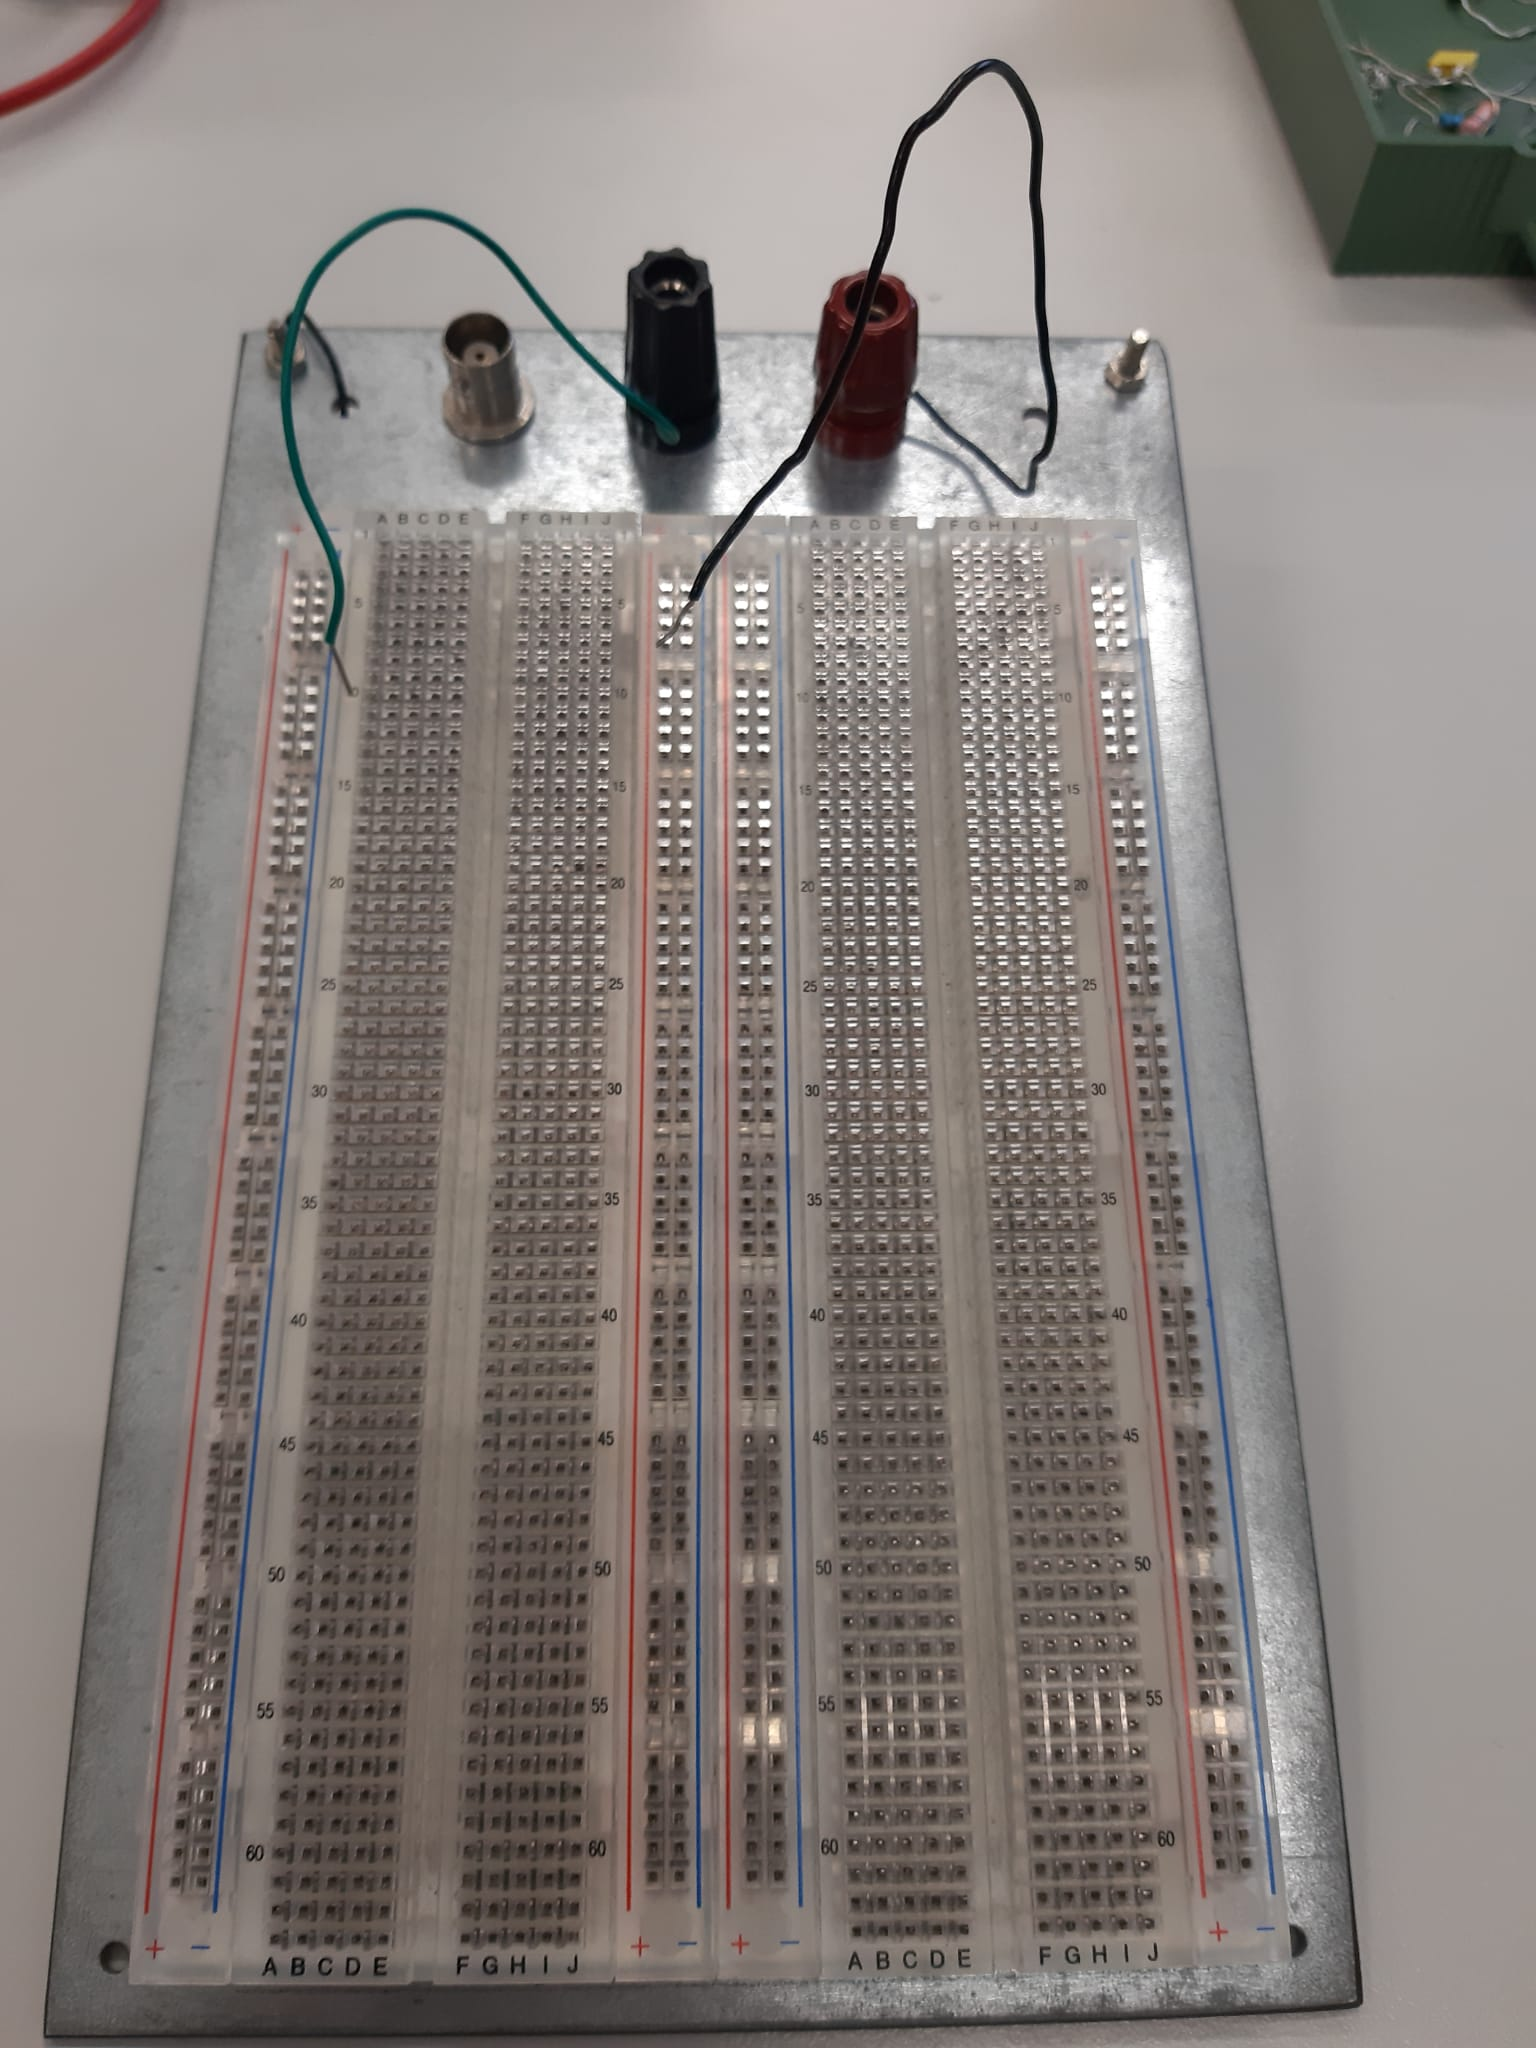
\includegraphics[scale=0.1]{Immagini/Circuitoooo.jpeg}
    \caption{}
\end{figure}

Lo strumento ci ha permesso di realizzare i circuiti su cui abbiamo condotto le diverse misure. Le componenti di circuito di cui ci siamo serviti sono state una resistenza, un condensatore, un induttore e un partitore resistivo, composto da boccole e da interruttori in grado di modificare la resistenza dello strumento.
Abbiamo fatto uso di un generatore di segnali ad onde quadre, delle quali era possibile modificare la tensione e l'offset, e di un oscilloscopio, in grado di misurare i segnali di tensione ai capi delle componenti.
Abbiamo articolato l'esperienza in 2 parti.
In primo luogo abbiamo studiato l'andamento della differenza di potenziale ai capi delle componenti di due differenti circuiti, sollecitati da un segnale ad onda quadra; nel primo caso ai capi di resistenza e capacità, nel secondo caso ai capi di resistenza ed induttanza.

Per lo studio dei circuiti RC ed RL abbiamo proceduto analizzando le equazioni differenziali associate, così da ottenere le relazioni tra le differenze di potenziale ai capi della resistenza ed il tempo.

Per il circuito RC, attraverso le leggi di Kirchhoff, siamo giunti alle equazioni differenziali. Per la scarica si trova
\begin{equation}
R\dot{I}+\frac{I}{C}=0
\end{equation}
mentre per la carica
\begin{equation}
    R\dot{Q}+\frac{Q}{C}=V_{0}
\end{equation}

Dalle quali abbiamo ottenuto le rispettive equazioni:

\begin{equation}
V_{R}(t)=-V_{0}e^{\frac{-t}{\tau}}
\end{equation}
\begin{equation}
    V_{R}(t)=V_{0}e^{\frac{-t}{\tau}}
\end{equation}

Dove $\tau$ è la costante di tempo caratteristica del circuito ed è definita come $\tau=RC$.

Per il circuito RL, attraverso le leggi di Kirchhoff, si giunge alle due equazioni differenziali per carica e scarica. Per la carica risulta essere

\begin{equation}
RI+L\dot{I}=V_{0}
\end{equation}
mentre per la scarica
\begin{equation}
    RI+L\dot{I}=0
\end{equation}

Risolvendo queste equazioni differenziali si giunge alle leggi che governano i due fenomeni, rispettivamente

\begin{equation}
V_{R}(t)=V_{0}\left[1-e^{\dfrac{-t}{\tau}}\right]
\label{eq. 7}
\end{equation}
\begin{equation}
    V_{R}(t)=V_{0}e^{\dfrac{-t}{\tau}}
    \label{eq.8}
\end{equation}

Dove $\tau$ è la costante di tempo caratteristica del circuito ed è definita come $\tau=\frac{L}{R}$.

Per quanto riguarda la seconda parte dell'esperienza si è proceduto in maniera analoga nello studio del circuito. Utilizzando i valori ricavati in precedenza per \textit{C} ed \textit{L}, abbiamo analizzato il circuito \textit{RLC} nei suoi tre diversi regimi, \textit{sottosmorzamento}, \textit{sovrasmorzamento} e \textit{smorzamento critico}.
Tali regimi possono essere idetificati grazie al rapporto tra le due costanti caratteristiche, ricavabili studiando la seguente equazione differenziale:

\begin{equation}
L\ddot{Q}+R\dot{Q}+\frac{Q}{C}=V_{0}
\end{equation}

Messa in luce l'analogia con l'equazione dell'oscillatore armonico smorzato, abbiamo riscritto l'equazione usando lo stesso formalismo:

\begin{equation}
\ddot{Q}+2\gamma\dot{Q}+\omega_{0}^{2}(Q-CV_{0})=0
\end{equation}

A seconda del valore di $\Delta=\gamma^{2}-\omega_{0}^{2}$ è, dunque, possibile identificare tre differenti regimi. La relazione che lega i parametri è
$$
\gamma=\dfrac{R}{2L}\qquad \omega_0 = \dfrac{1}{\sqrt{LC}}
$$

Per il regime sottsomorzato $\gamma<\omega_{0}$,
per il regime sovrasmorzato $\gamma>\omega_{0}$,
per il regime di smorzamento critico $\gamma=\omega_{0}$.
